% This is LLNCS.DEM the demonstration file of
% the LaTeX macro package from Springer-Verlag
% for Lecture Notes in Computer Science,
% version 2.4 for LaTeX2e as of 16. April 2010
%
\documentclass{llncs}
%
\usepackage{makeidx}  % allows for indexgeneration
\usepackage{graphicx} % so we can include images
\usepackage[utf8]{inputenc} % display all characters properly
\usepackage[unicode=true,english,american]{babel} % doesn't change anything?

\usepackage{url}
\usepackage{listings} % for listing code
\usepackage{color} % colors are nice

\definecolor{black}{rgb}{0,0,0}
\definecolor{gray}{rgb}{0.6,0.6,0.6}
\definecolor{white}{rgb}{1,1,1}

\definecolor{keywords}{rgb}{0.5,0,0.6}
\definecolor{strings}{rgb}{0,0.4,0}
\definecolor{comments}{rgb}{0.5,0.5,0.5}

\lstset{ %
  language=Java,                  % the language of the code
  basicstyle=\ttfamily\footnotesize,       % the size of the fonts that are used for the code
  numbers=left,                   % where to put the line-numbers
  numberstyle=\tiny\color{gray},  % the style that is used for the line-numbers
  stepnumber=1,                   % the step between two line-numbers. If it's 1, each line 
                                  % will be numbered
  numbersep=5pt,                  % how far the line-numbers are from the code
  backgroundcolor=\color{white},  % choose the background color. You must add \usepackage{color}
  showspaces=false,               % show spaces adding particular underscores
  showstringspaces=false,         % underline spaces within strings
  showtabs=false,                 % show tabs within strings adding particular underscores
  frame=single,                     % adds a frame around the code
  rulecolor=\color{black},        % if not set, the frame-color may be changed on line-breaks within not-black text (e.g. comments (green here))
  tabsize=2,
  captionpos=b,                   % sets the caption-position to bottom
  breaklines=true,
  breakatwhitespace=true,
  %title=\lstname,                 % show the filename of files included with \lstinputlisting;
  keywordstyle=\color{keywords},
  commentstyle=\color{comments},
  stringstyle=\color{strings},
  %escapeinside={\%*}{*)},        % if you want to add LaTeX within your code
  %morekeywords={*,...},          % if you want to add more keywords to the set
  %deletekeywords={}           % if you want to delete keywords from the given language
}

%
\begin{document}
%
\frontmatter          % for the preliminaries
%o
\pagestyle{headings}  % switches on printing of running heads
\addtocmark{Code Generation From ECDAR} % additional mark in the TOC
%
\mainmatter              % start of the contributions
%
\title{Code Generation From ECDAR}
%
\titlerunning{Code Generation From ECDAR}  % abbreviated title (for running head)
%                                     also used for the TOC unless
%                                     \toctitle is used
%
\author{Rasmus Berntsen \and Florian Biermann \and Lauge Groes \and Nicolas Wainach Lundqvist Jensen \and Thomas Kokholm \and Piort Stawiski \and Wiktor Michal Zdziechowski}

\authorrunning{Rasmus Berntsen et al.} % abbreviated author list (for running head)

%%%% list of authors for the TOC (use if author list has to be modified)
\tocauthor{Rasmus Berntsen, Florian Biermann, Lauge Groes, Nicolas Wainach Lundqvist Jensen, Thomas Kokholm, Piort Stawiski, Wiktor Michal Zdziechowski}

\institute{IT University of Copenhagen, Denmark\\
\email{\{raber, fbier, lgro, nicl, tkok, psta, wmic\}@itu.dk}
}
\maketitle % typeset the title of the contribution

\begin{abstract}

\end{abstract}

\section{Introduction\label{introduction}}
\input{introduction}



%%% Begin of background

\section{Background\label{background}}
%% BACKGROUND (Wiktor) %%% 

% LAST UPDATE: applying changes from Andrzej's comments (27.11.2012) % 


\subsection{Timed Input/Output Automata \label{background-tioa}}
%
The "Timed Input/Output Automata" is a basic, mathematical specification framework for description and analysis of real time systems. 
In this framework, system is represented by nondeterministic, possibly infinite-state, state machine referred 
as “timed I/O automaton” (TIOA) \cite{Kaynar:2006:TTI:1203437}. TIOA has been implemented as the modeling language in ECDAR \cite{conf/atva/DavidLLNW10}.

\begin{figure}[t]
\label{simple-model}
\begin{centering}
\includegraphics[scale=0.7]{images/bev_machine_model}
\par\end{centering}
\caption{Model of beverage-serving machine.}
\label{bev-machine}
\end{figure}

The preceding figure (see fig. \ref{bev-machine}) illustrates the model of beverage-serving machine. Given a coin (\emph{coin}), it serves either coffee (\emph{cof}) 
or tea (\emph{tea}) within a given time interval. Moreover, free tea is served once in awhile. In the example, the TIOA consists of and two locations represented by 
circles: \emph{Idle} and \emph{Serving}. \emph{Idle} represents the starting location, and the state of machine waiting for coin input (\emph{coin?}).  
 The flow of TIOA is controlled by three types of labels: \emph{invariants}, \emph{guards} and \emph{clock-reset operations}. 
Invariants are defined on locations ($y\leq 6$) and represent constraints for the clocks in order for the control to remain in particular location until time requirement is fulfilled.  
Guards are located on the edges ($y\geq 2$ and $y\geq 4$) and express conditions on the values of clock that must be satisfied in order for 
the edge to be taken. When the condition is satisfied, the transition occurs and action (\emph{cof!} or \emph{tea!}) is triggered. Clock-reset operations ($y=0$) are simple
clock value manipulations in form of assignment that enforce progress in the system.

In ECDAR, the specification interface is leveraging the UPPAAL TIGA language \cite{behrmann_uppaal-tiga:_2006} to describe TIOA. However, the following constraints are retained\footnote{See \href{http://people.cs.aau.dk/adavid/ecdar/examples.html\#lang}}:   
%
\begin{itemize}
\item Invariants may not be strict.
\item Inputs must use controllable edges.
\item Outputs must use uncontrollable edges.
\item All channels must be declared broadcast.
\item The system is implicitly input enabled due to broadcast communication but for refinement checking purposes the relevant inputs must be explicit in the model.
\item In the case of parallel composition of several components, a given output must be exclusive to one component.
\item For implementations, outputs must be urgent.
\item For implementations, every state must have independent time progress, i.e., progress must be ensured by either an output or infinite delay.
\item $\tau$-transitions (no output or input) are forbidden. %There was a comment about this item%
\item Global variables are forbidden.
\end{itemize}

\subsection{Code Generation \label{background-codegeneration}}
In order to clarify what code generation is one need to understand what a model transformation is, as this is a fundamental part of code generation. In short one could say that the model transformation is a way to ensure that the final code is consistent and with a reduced number of errors. The generation is an automated way to produce code from models. The actual generation is defined by the software developer, thus it is defined what the output should be, but the input and the data is not.

There is generally two ways to do model transformations, that is model to model and model to text, the former known as M2M and the latter M2T. There are also a lot of other tools and techniques for transformation, which should not be confused with model transformations. One could mention an XSLT-transformation as an example, where the base input is an XML-document and the final output is another XML-document, often XHTML, with a predefined XML-Schema.

Model to model is a transformation of a number of models to a given number of new models - from X number of models to Z number of new models. Model to text is the transformation of a number of models to text, the text could for instance be code - which is why the process sometimes is known as model to code.




%%% End of background

%%% Begin of implementation

\section{Implementation\label{implementation}}
The proposed implementation of the ECDAR code generator is split up
in two parts. The first part is a framework of abstract classes, implementing
in as much detail as possible the single parts of ECDAR specifications
(i.e. edges, locations, TIOA). The second is the actual code generation.
Our code generator generates sources which inherit from the abstract
framework to minimize the amount of code that needs actually to be
generated. This means that nearly all design decisions have been made
prior to generating code, reducing space for possible errors. This
section describes our implemented subset of ECDAR and the code generator
in detail. 


\subsection{Presumptions and Resulting Motivations\label{implementation-presumptions}}

Our implementation represents only a subset of actual ECDAR. Currently,
the implementation assumes only one clock per automaton. Also, we
assume the specification to be valid, since there are other tools
that verify correctness%
\footnote{\href{}{http://people.cs.aau.dk/adavid/ecdar/}%
}.

Additionally, the only operator we implement is the parallel composition
operator. Let $M$ be the type ECDAR specification. Then all operators
in ECDAR are of type $M\rightarrow M\rightarrow M$. Other than for
the majority of operators, which refine the specification, it is impractical
to implement parallel composition as a model-to-model transformation,
since it produces the cross-product of two models. \cite{david_compositional_2012}
These models are size $|M|^{2}$ and generating code for them would
consume a large amount of memory and complexity. This would be inappropriate
for an embedded system. We elaborate on this further in Sec. \ref{implementation-framework}.

ECDAR specifications are written on the assumption of the synchrony
hypothesis (see Sec. \ref{background-ecdar}). \cite{david_compositional_2012}
This is an important property for code generation, as reasoning about
time differences in execution becomes unnecessary for the developer.
However, we still kept overhead low to achieve reasonable fast performance.

To produce feasible code that would be able to run on embedded systems,
we targeted Real-Time Java (Java RTS)%
\footnote{\href{}{http://www.oracle.com/technetwork/java/javase/tech/index-jsp-139921.html}%
}. Java RTS was designed to improve upon standard Java in terms of
timing accuracy an real-time embedded systems.


\subsection{The ECDAR Framework \label{implementation-framework}}

\begin{figure}
\begin{centering}
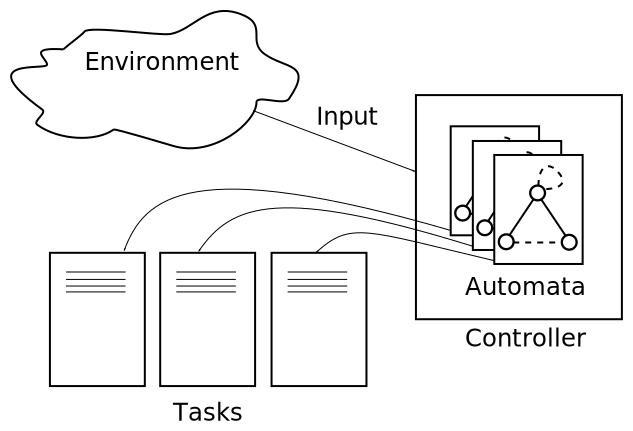
\includegraphics[scale=0.5]{images/ecdar_architecture}
\par\end{centering}

\caption{Schematic of the architecture of our ECDAR implementation.}
\end{figure}


The architecture we chose is based upon Amnell et al.\cite{amnell_code_2002}
with some modifications. Communication between automata happens through
input generated by uncontrollable edges -- there are no shared variables
(see Sec. \ref{background-tioa}). Input is processed by a controller
object, which initializes automata and notifies automata about input.

We require multiple automata to execute in quasi-parallel. Therefore,
we do not queue tasks. Since the automata are moved to classical threading
architecture, we do not require multiple processor units. Instead,
the controller and each automaton run in separate threads. Since there
is no communication between automata directly, we can minimize synchronizing
so that nearly no waiting is required.

The following overview will give further implementation details on
each component of ECDAR as we implemented it:


\subsubsection{Locations}

Each location is a associated with a task. Task execution is moved
to a separate thread. Location is implemented as a class holding an
array of controllable and uncontrollable edges that point away from
it.


\subsubsection{Edges}

An edge holds a reference to the location which the parent automaton
will be at after traversing this very edge. Edges can be asked if
they will be available at a given time. This is implemented to enable
lazy waiting in the automaton's traversal checker. Each edge is associated
with some input. If an edge is controllable, it will be triggered
if the automaton is notified at this input. If it is uncontrollable,
it will send its input to the controller. Furthermore, edges have
access to the clock of the parent automaton to reset it appropriately.

The implementation makes a class-wise distinction between controllable
and uncontrollable edges and hard-codes the behavior for given input.
Such hard-coded features are e.g. notifying the controller on traversing
an uncontrollable edge.


\subsubsection{TIOA}

The implementation of timed I/O automata holds a set of locations
and a reference to the location it is currently at. The TIOA is executed
by a thread that keeps checking for available edges and traverses
along these, as soon as they become enabled. To check if an edge is
available, let $E_{s\rightarrow t}$ be an edge where $s,\, t$ are
start and target locations respectively. Furthermore, let $g(E)$
be a function evaluating the guard of an edge $E$ and $I(l)$ a function
evaluating the invariant of a location $l$. Our implementation uses
$g'(E_{s\rightarrow t})=g(E_{s\rightarrow t})\wedge I(t)$ to check
if $E_{s\rightarrow t}$ is available.

Additionally, the automaton has the ability to return the current
local clock state (see \ref{implementation-presumptions}) and to
reset the clock. We use the same notion of clocks as \cite{amnell_code_2002},
where time on the local clock is the difference between the current
time on the system clock and the time the local clock was started.
Resetting the local clock means to use the current system clock time
as the new start time.


\subsubsection{Controller}

The controller holds all automata given in the specification, executes
them initially in quasi-parallel and notifies automata about input
from the environment. It is a singleton, accessible in a static fashion.
This property is useful for uncontrollable edges that need to notify
the controller about input.


\subsection{Walk-through Example}

% We may need an example specification here, some two-locations-two-edges thingy.


\subsection{Code Generation \label{implementation-code-generation}}

*Draft* 

In our implementation we generate executable Java code based on ECDAR models. The method we chose to use is the model-to-text transformation method.


We chose to use model-to-text instead of model-to-model transformations
because of the complexity (a lot of meta classes) and also because
of the limited scope of the project. % Rewrite this!


%%% End of implementation

\section{Evaluation and Discussion}
\subsection{Testing}
\label{Testing}
In order to test our software solution three different testing methods have been
arranged.

\subsubsection{Compiling properly}
Making sure every output compiles properly.

\subsubsection{Logfile testing}
For the project an logfile analysis program have been incorporated. A small
program verifying that the signals in the generator code are fired in the right
order according to the input model.  The analysis program is hardcoded to match
our testing model (see Fig. \ref{simple-model}). Thus it is checking for signals
like: GRANT, COIN and TEA, in the specifyied order. If a signal is called within
the generator before it is supposed too (e.g TEA before COIN) the analysis
program will call for an ERROR.

The logfile contain timestamps of global time from each atomaton in a model. The
global time can then be verified by comparison with time assigned within the
ECDAR modelling tool.

\subsubsection{Manual Comparison}
Final testing procedure is a manual step-by-step comparison of a simple
graphical atomaton model and the corisponding code generated. Cycling through
the times, comparing each step with the output.
%(verified by Andrzej Wasowski).

\subsection{Presumptions and Resulting Motivations}
\label{implementation-presumptions}

Our implementation represents only a subset of actual ECDAR. Currently, the
implementation assumes only one clock per automaton. Also, we assume the
specification to be valid, since there are other tools that verify
correctness\footnote{\url{http://people.cs.aau.dk/adavid/ecdar/}}.

The only operator we implement for code generation is the parallel
composition operator. Let $M$ be the type ECDAR specification. Then
all operators in ECDAR are of type $M_{i}\otimes M_{j}\rightarrow M_{ij}$.
Other than for the majority of operators, which refine the specification,
it is impractical to implement parallel composition as a model-to-model
transformation, since it produces the cross-product of two models
\cite{david_compositional_2012}. These models are size $|M_{i}|\cdot|M_{j}|$
and generating code for them would consume a large amount of memory
and raise complexity. This would be inappropriate for an embedded
system. We elaborate on this further in Sect. \ref{implementation-framework}.

ECDAR specifications are written on the assumption of the synchrony
hypothesis (see Sect. \ref{background-ecdar}) \cite{david_compositional_2012}.
This is an important property for code generation, as reasoning about
time differences in execution becomes unnecessary for the developer.
However, we still kept overhead low to achieve reasonable fast performance.

%To produce feasible code that would be able to run on embedded systems,
%we targeted Real-Time Java (Java RTS)%
%\footnote{\href{}{http://www.oracle.com/technetwork/java/javase/tech/index-jsp-139921.html}%
%}. Java RTS was designed to improve upon standard Java in terms of
%timing accuracy an real-time embedded systems.






\section{Related Work\label{related}}
ECDAR is a TIOA modeler based on UPPAAL. A similar tool based on UPPAAL already exists. 

\paragraph{Times}
Times\footnote{\href{http://www.timestool.com}} is a tool for modeling and implementation of embedded systems. Times is a graphical simulator, in which a user can validate dynamic behavior of a system and see how tasks execute - much like Ecdar, but it can also do code-generation. However there is a difference between Ecdar and Times.

Looking at what are taking as input by the controller - Times simple takes a model and generates code. ECDAR: Synthesize models for you so to avoid “that” stage. In ECDAR you have the possibility to you use composition.

\paragraph{Composable Code Generation for Model-Based Development}
by Kirk Schloegel et al. present a framework for generating code\cite{composable-code-generation}. They emphasize how utilizing their framework, code generators aren't programs seperated from a correspnding graphical model as it often have been in the past. Our code generator isn't based on this framework, however their approch on developing code generators with focus on graphical models is related to our apporch with ECDAR. 

\paragraph{Code Synthesis for Timed Automata}
by Tobias Amnell et al. present a framework for the development of real-time embedded
systems\cite{Amnell:2002:CST:779110.779112}. Their work is sumulor to our project. In the article the illustrate how their framework is based on timed automatas and real-time tasks - relative to our concept with ECDAR.



\section{Conclusion}
\input{conclusion}

%
...
%

% ---- Bibliography ----
\bibliographystyle{plain}
\nocite{*}
\bibliography{MDD}

% Add more references to MDD.bib by hand or send links with them to me, I'll generate the file properly then. /Florian
%
%\begin{thebibliography}{5}

%\bibitem {Selic:PoMDD}
%\textsl Bran Selic: {The Pragmatics of Model-Driven Development}, IBM Rational Software, (2003), \url{http://ieeexplore.ieee.org/stamp/stamp.jsp?tp=&arnumber=1231146}
%\bibitem {Ecdar:Ewe}
%\textsl Environment for Compositional Design and Analysis of Real Time Systems (2012-10-19), \url{http://ecdar.cs.aau.dk/}
%\bibitem {Larsen:UPPAAL}
%\textsl Larsen, K., Pettersson, P., Yi, W.: Uppaal in a nutshell. International Journal on Software Tools for Technology Transfer (STTT) 1(1), 134–152 (1997)


%\end{thebibliography}

%
\appendix
\section{First Appendix}

\end{document}
